\chapter{Results}

By expanding the microarchitecture from Exercise 1 \cite{compendium} with a forwarder, pipeline registers, hazard detection and improved ALU, PC and control modules, we succeded in implementing a pipelined, multi-cycle, MIPS-like processor.
Each component was tested with individual testbenches.
The system as a whole was tested using an end-to-end testbench, as well as by uploading the bitfile to an FPGA in the lab and verifying correctness using the \texttt{hostcomm} utility.
We succeded in implementing support for the instructions listed as requirements in the exercise description.

\section{Testing on the FPGA}

\begin{figure}[h!]
    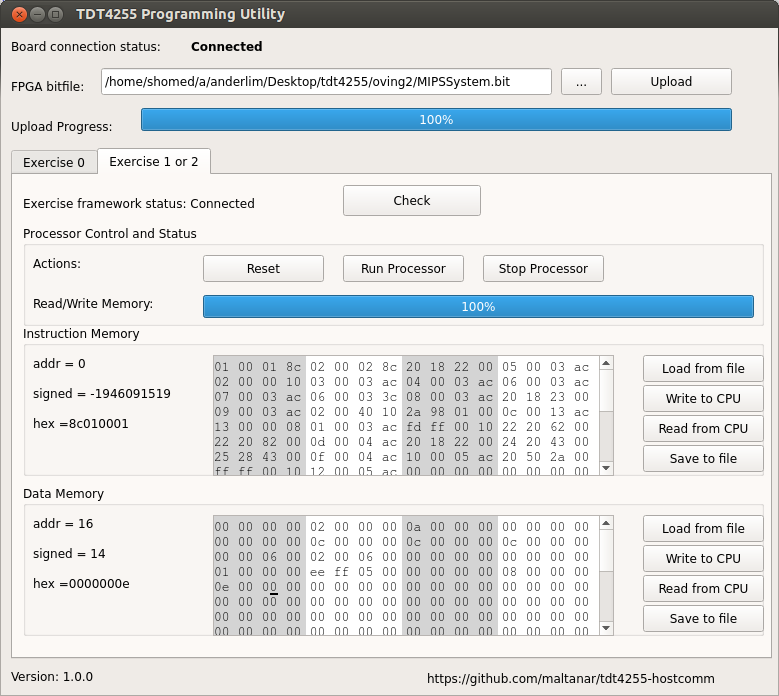
\includegraphics[width=\linewidth]{img/hostcomm_result.png}
    \caption{A screenshot of the hostcomm utility after allowing our processor to execute a the test program.}
    \label{fig:hostcomm}
\end{figure}